% !TeX encoding = UTF-8
\documentclass[aspectratio=169]{beamer}
\useoutertheme[progressbar=frametitle]{metropolis}
\useinnertheme{metropolis}
\definecolor{nabgray}{rgb}{0.6,0.59,0.61}
\usecolortheme[named=nabgray]{structure}

\usepackage{tikz}
\usepackage[utf8]{inputenc}
\usepackage[spanish]{babel}
\usepackage{fontspec}
\setmonofont{JetBrains Mono}
\setmainfont{Roboto}
\setsansfont{Roboto}

\usepackage{smartdiagram}
\usepackage{qtree}
\usepackage{verbatim}
\usepackage{svg}
\usepackage{graphicx}
\usepackage{color}

\definecolor{lightgray}{rgb}{0.95, 0.95, 0.95}
\definecolor{darkgray}{rgb}{0.4, 0.4, 0.4}
%\definecolor{purple}{rgb}{0.65, 0.12, 0.82}
\definecolor{editorGray}{rgb}{0.95, 0.95, 0.95}
\definecolor{editorOcher}{rgb}{1, 0.5, 0} % #FF7F00 -> rgb(239, 169, 0)
\definecolor{editorGreen}{rgb}{0, 0.5, 0} % #007C00 -> rgb(0, 124, 0)
\definecolor{orange}{rgb}{1,0.45,0.13}
\definecolor{olive}{rgb}{0.17,0.59,0.20}
\definecolor{brown}{rgb}{0.69,0.31,0.31}
\definecolor{purple}{rgb}{0.38,0.18,0.81}
\definecolor{lightblue}{rgb}{0.1,0.57,0.7}
\definecolor{lightred}{rgb}{1,0.4,0.5}
\usepackage{upquote}
\usepackage{listings}
\lstset{language=java,
	basicstyle=\footnotesize\ttfamily,
	keywordstyle=\footnotesize\color{blue}\ttfamily,
	escapeinside={<@}{@>}
}
\lstdefinelanguage{Kotlin}{
	comment=[l]{//},
	commentstyle={\color{gray}\ttfamily},
	emph={delegate, filter, first, firstOrNull, forEach, lazy, map, mapNotNull, println, return@},
	emphstyle={\color{purple}},
	identifierstyle=\color{black},
	keywords={abstract, actual, as, as?, break, by, class, companion, continue, data, do, dynamic, else, enum, expect, false, final, for, fun, get, if, import, in, interface, internal, is, null, object, override, package, private, public, return, set, super, suspend, this, throw, true, try, typealias, val, var, vararg, when, where, while},
	keywordstyle={\color{lightblue}\bfseries},
	morecomment=[s]{/*}{*/},
	morestring=[b]",
	morestring=[s]{"""*}{*"""},
	ndkeywords={@Inject, @Deprecated, @JvmField, @JvmName, @JvmOverloads, @JvmStatic, @JvmSynthetic, Array, Byte, Double, Float, Int, Integer, Iterable, Long, Runnable, Short, String},
	ndkeywordstyle={\color{orange}\bfseries},
	sensitive=true,
	stringstyle={\color{olive}\ttfamily},
}

\usebackgroundtemplate%
{%
	
\includegraphics[width=\paperwidth]{Images/Contenido}%
}


\title{Serverless con el proyecto Fn}
\author{Víctor Orozco}
\institute{Nabenik}
\date{\today}

\begin{document}





{
    \usebackgroundtemplate{
\includegraphics[width=\paperwidth]{Images/portada}}
    \setbeamercolor{frametitle}{fg=red}
    \usebeamercolor[fg]{normal text}
    \frame{\titlepage}
}


\begin{frame}{Serverless}
\begin{figure}
	\centering
	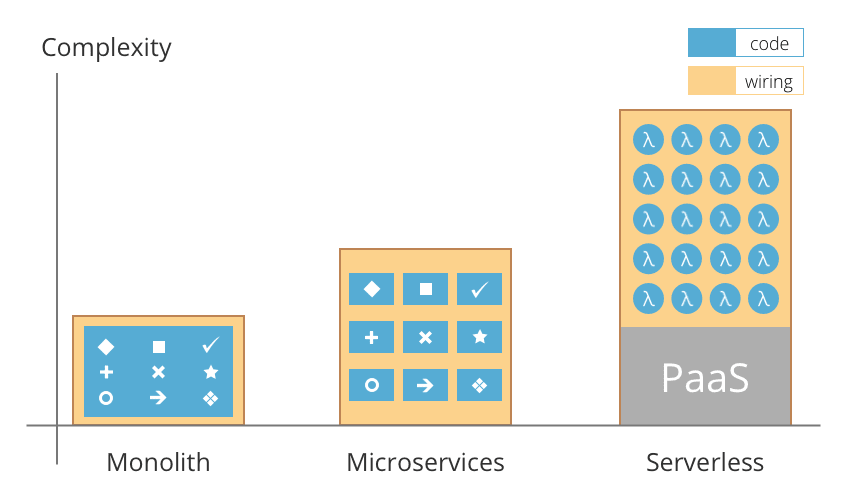
\includegraphics[width=0.8\linewidth]{Images/serverlessevolution.png}
	\label{fig:kotlin}
\end{figure}
\end{frame}


\begin{frame}{Tendencias}
\begin{figure}
	\centering
	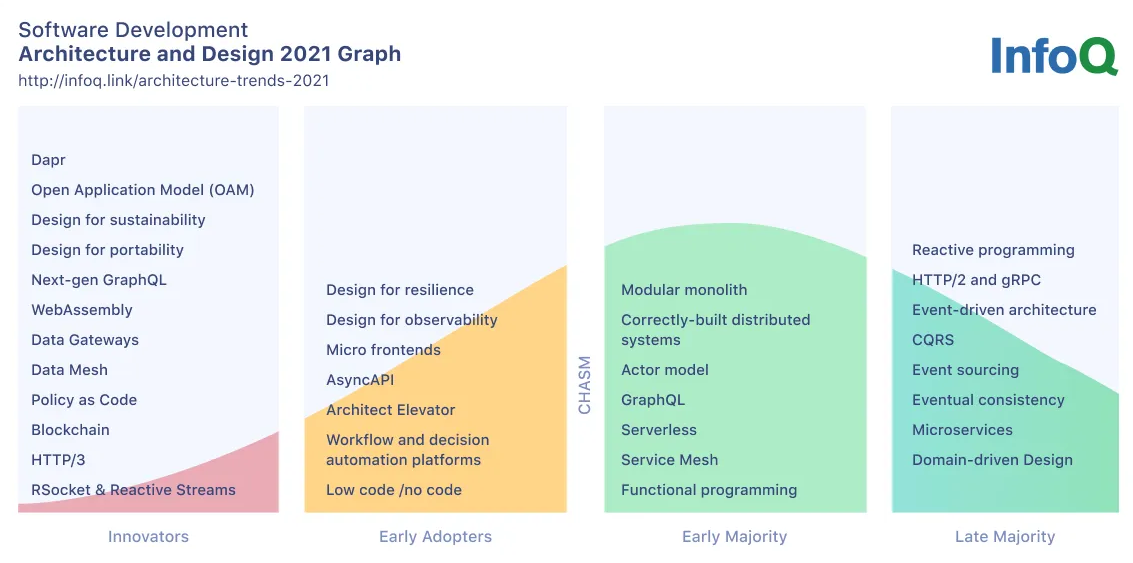
\includegraphics[width=0.9\linewidth]{Images/trends.png}
	\label{fig:trends}
\end{figure}
\end{frame}



\begin{frame}{Idea general}
\begin{figure}
	\centering
	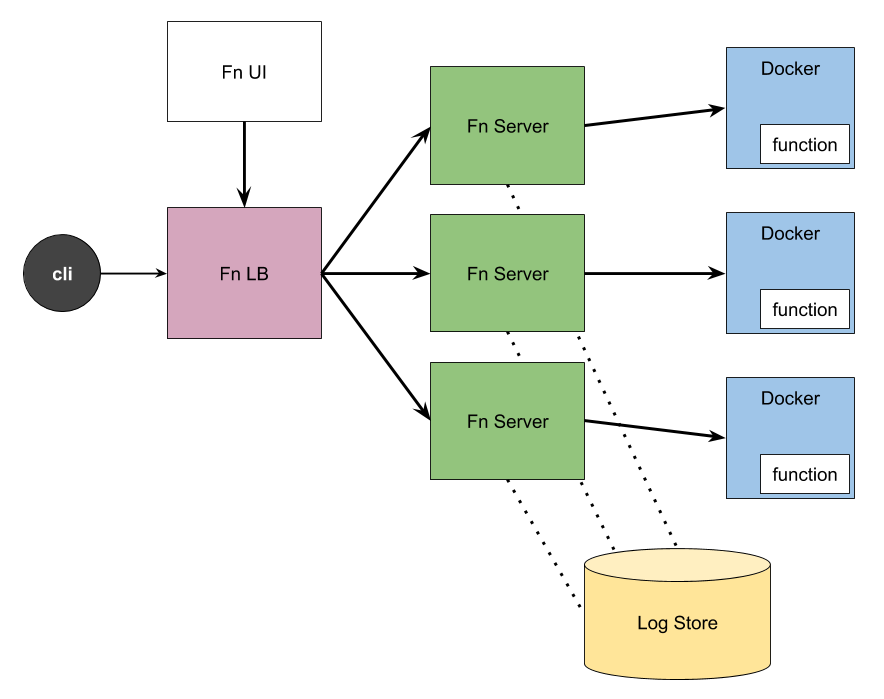
\includegraphics[width=0.7\linewidth]{Images/fn-architecture.png}
	\label{fig:architecture}
\end{figure}
\end{frame}



\begin{frame}{Idea general}
\begin{exampleblock}{Serverless}

Serverless architectures are application designs that incorporate third-party “Backend as a Service” (BaaS) services, and/or that include custom code run in managed, ephemeral containers on a \textbf{“Functions as a Service” (FaaS) platform.}
\end{exampleblock}
Martin Fowler
\end{frame}

\begin{frame}{BaaS}
\begin{figure}
	\centering
	
\includegraphics[width=0.9\linewidth]{Images/baas.png}
	\label{fig:baas}
\end{figure}
\end{frame}


\begin{frame}{FaaS}
Backend

\begin{itemize}
\item Zip
\item Docker
\item Propietario
\end{itemize}

Trigger
\begin{itemize}
\item Http
\item Cron
\item Evento Cloud
\end{itemize}
\end{frame}

\begin{frame}{Closed FaaS}
\begin{figure}
	\centering
	
\includegraphics[width=0.9\linewidth]{Images/closedfaas.png}
	\label{fig:closedfaas}
\end{figure}
\end{frame}

\begin{frame}{Serverless}
	\begin{columns}[T] % contents are top vertically aligned

		\begin{column}[T]{6cm} % alternative top-align that's better for graphics
Ventajas
		\begin{enumerate}
		\item Costos
		\item Velocidad de desarrollo
		\item Amigable con el planeta
        \item Escalabilidad
		\end{enumerate}
		\end{column}
		\begin{column}[T]{6cm} % each column can also be its own environment
Desventajas
        \begin{enumerate}
        \item Curva de aprendizaje
        \item Lock-in
        \item Cold start
        \item Control
        \end{enumerate}

		\end{column}
	\end{columns}
\end{frame}

\begin{frame}{Open Source FaaS}
\begin{figure}
	\centering
	
\includegraphics[width=0.9\linewidth]{Images/open-faas.png}
	\label{fig:faas}
\end{figure}
\end{frame}

\begin{frame}{Proyecto fn}
\begin{figure}
	\centering
	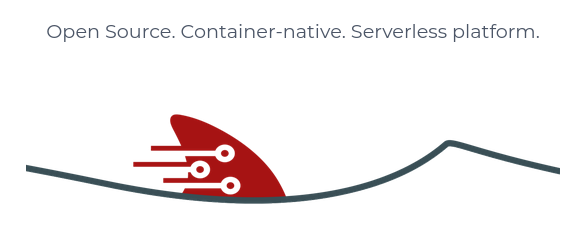
\includegraphics[width=0.5\linewidth]{Images/fn.png}
\end{figure}

\begin{enumerate}
        \item Open Source
        \item Docker
        \item Políglota
        \item On Prem, Oracle Cloud Functions
\end{enumerate}

\begin{figure}
	\centering
	
\includegraphics[width=0.5\linewidth]{Images/langs.png}
\end{figure}
\end{frame}


\begin{frame}{Demo}
	\begin{enumerate}
		\item Java FDK
        	\begin{enumerate}
        		\item Aplicación
        		\item Función
                \item Trigger (Ejecución)
        	\end{enumerate}
		\item On Prem (Docker)
        \item Oracle Cloud Functions
	\end{enumerate}
    {\scriptsize \url{https://medium.com/oracledevs/extend-your-api-with-serverless-functions-and-api-gateways-2a383561ef5c}}
    
\end{frame}

\begin{frame}{Víctor Orozco}
    \begin{columns}[T] % contents are top vertically aligned

        \begin{column}[T]{4cm} % alternative top-align that's better for graphics
            \begin{figure}
                \centering
                
\includegraphics[width=\linewidth]{Images/logos}
            \end{figure}
        \end{column}
        \begin{column}[T]{6cm} % each column can also be its own environment
            \begin{itemize}
                \item vorozco@nabenik.com
                \item \href{https://twitter.com/tuxtor}{@tuxtor}
                \item \href{http://vorozco.com}{http://vorozco.com}
                \item \href{http://tuxtor.shekalug.org}{http://tuxtor.shekalug.org}
            \end{itemize}
            \begin{center}
                
\includegraphics[width=0.1\linewidth]{Images/cclogo}
                \\
                This work is licensed under Creative Commons Attribution-NonCommercial-ShareAlike 3.0 Guatemala (CC BY-NC-SA 3.0 GT).
            \end{center}
        \end{column}
    \end{columns}
\end{frame}



\end{document}
